\chapter{Testing script}
Testing script is one of the core of testing framework.
A testing script can be called a test case.
This chapter describes the components that make up a testing script. At the end of chapter, there are some examples of testing scripts I use for experiments in Chapter \ref{ch:experiments}.

\section{Testing script structure}
\label{sec:script_comp}
A testing script consists of one or more script actions. By running the sequence of actions, the goal of the test can be achieved by asserting the result obtained during or end of the test case. Each script action has the following elements:
    \begin{itemize}
		\item[--] \textbf{Source object}: element on the screen to be applied action on which is detected in Chapter \ref{ch:screen_recognize}.
		\item[--] \textbf{Action}: what to do with source object, will be covered in Section \ref{sec:actions}.
		\item[--] \textbf{Execution time}: how long it takes to complete the action. This parameter is used for delaying the screen reading process while the robot is running.
		\item[--] \textbf{Expected object} (optional, depended on each action): after finishing action, what expected to be display on the screen. This is the goal of the verification step.
	\end{itemize}

\subsection{Actions}
\label{sec:actions}
The robot is designed for physically contacting with the phone. It simulates human operations to perform testing process.
Although there are many complicated actions people can make, these actions can be classified into 4 basic actions that the robot can apply on mobile phone screen:

    \begin{itemize}
		\item[--] \textbf{Click}: perform a quick single tap on screen
		\item[--] \textbf{Hold}: tap and keep pointer on the screen for a short time then release. This action is usually used for calling context menu.
		\item[--] \textbf{Drag}: tap on the screen, move pointer to a certain location then release. This action can be used for dragging an item to another location or scrolling a list.
		\item[--] \textbf{Flick}: tap on the screen and quickly move pointer apart and release. Flicking helps user to scroll a list faster.
	\end{itemize}

\subsection{States of system}
The states of the system is illustrated in Figure \ref{fig:system_state}.

    \begin{figure}[H]
		\centering
		\includegraphics[scale=0.7]{Chapters/Fig/system_state.png}
		\caption{System state diagram}
		\label{fig:system_state}
	\end{figure}

While in operation, the system tends to find the target object for calling the action. If the Image Processor returns no such object, the test case fails.

Once the target is found, appropriate action is applied to as in the script. After finishing, the result on the screen continues to be used for next action in sequence.

The process is repeated until no more action in the script. After this stage, the result of the test case is ``success''. If there is any failure during testing process, the test case will be interrupted and produce failing message.

\subsection{System sequence diagram}
From System state diagram, a Sequence diagram with specific actors is derived. Figure \ref{fig:sequence_diagram} shows a compact sequence of a testing process.

To begin a test, the user needs to set up parameters of the testing device. These parameters are necessary for converting pixel location on the display to the real location on the phone screen.

Afterward, Script Actions are generated. The director of the system, Phone Test System, receives the list of Script Actions, and repeatedly check if corresponding Image Object exists in the content of the screen via Image Processor's operations. If the required object is not found, the sequence stops with ``fail'' result. Otherwise, the script continues with creating Robot Action which is determined in Script Action. Phone Test System then calls \textit{execute} method of Robot Action to have the robot running.

After execution finishes, if an expected object is specified in the action script, Image Processor reads the screen again and verifies whether that object exists or not.

This process is replicated along the actions in the script. Whenever there is an missing object, the test fails. If walking through all actions in the test script, the final result is display on the application user interface.

    \begin{figure}[H]
		\centering
		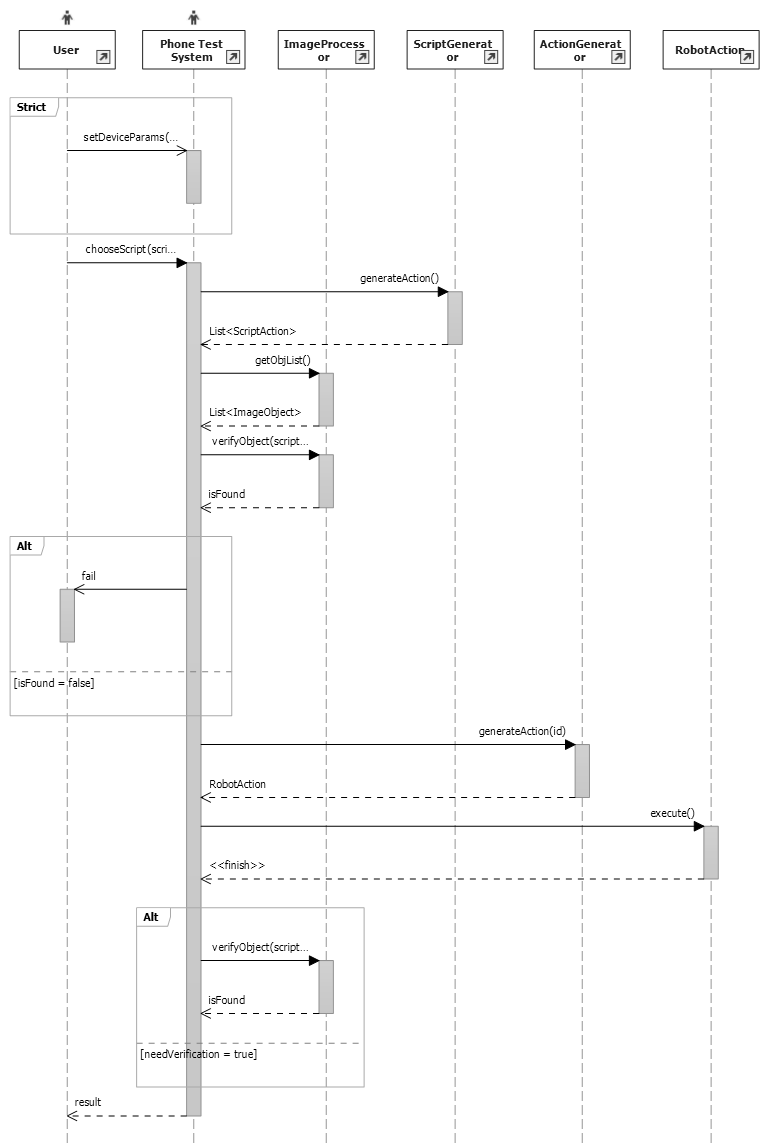
\includegraphics[scale=0.75]{Chapters/Fig/sequence_diagram.png}
		\caption{System sequence diagram}
		\label{fig:sequence_diagram}
	\end{figure}

\section{Testing script example}
\label{sec:eg_script}
This section illustrates some test cases and describes the schema in detail. The schema is then used for making test script by system's components described in Chapter \ref{ch:implement}.

\subsection{Simple click test}
This is the most simple test case. The schema is described in following flow diagram.
	\begin{figure}[H]
		\centering
		\includegraphics[scale=0.55]{Chapters/Fig/click_test_diag.png}
		\caption{Simple Click Test flow diagram}
		\label{fig:click_test_diag}
	\end{figure}

In this test case, the robot will search for a simple button named READY and the perform a click on it. After that, a SUCCESS button appears in different position on the screen. The robot will move to that button's location to click on it. When this sequence finishes, the screen will display the READY button again.
This test case is useful for testing the movement of the robot.

\subsection{Set alarm test}
This is more complicated test case. In this schema, the robot will perform an alarm setting scenario where it will change the current alarm at 8:30 AM to 11:30 AM. Flow diagram of script is presented below:

	\begin{figure}[H]
		\centering
		\includegraphics[scale=0.55]{Chapters/Fig/alarm_test_diag.png}
		\caption{Set Alarm Test flow diagram}
		\label{fig:alarm_test_diag}
	\end{figure}

To walk though this test case, the system has to find an item labeled ``8:30 AM'' to click on. After that, a new screen is displayed with the new target named ``Time''. By clicking on Time item, a time selecting dialog is popped up. The robot has to drag ``8'' item up to make the hour be ``11''. Then, to finish setting alarm, OK and DONE buttons is pressed sequentially. If the final screen display correct ``11:30 AM'' alarm item, the test case is supposed to be passed.